\documentclass[aspectratio=169, 11pt, t, xcolor={table}]{beamer}
% Slides of the English course "Computer Architecture" (same theme as the
% ENSB decks: light background, teal + orange). Compile from en/slides/.
\usepackage{amsmath, amssymb}
\usepackage{booktabs, colortbl, tabularx, array}
\usepackage{tikz}
\usepackage[skins]{tcolorbox}
\usepackage{fontawesome5}
\usepackage{listings}
\usepackage{fontspec}
\usetikzlibrary{positioning, calc, arrows.meta, shapes.geometric, decorations.pathreplacing}

\setsansfont{texgyreheros}[Extension=.otf, UprightFont=*-regular, BoldFont=*-bold,
    ItalicFont=*-italic, BoldItalicFont=*-bolditalic]
\newfontfamily\codefont[Scale=0.95, BoldFont=lmmonolt10-bold.otf,
    ItalicFont=lmmono10-italic.otf]{lmmono10-regular.otf}

\definecolor{brandTeal}{HTML}{5CC8E6}
\definecolor{brandOrange}{HTML}{FFA27F}
\definecolor{brandLight}{HTML}{F8F9FA}
\definecolor{brandDark}{HTML}{263238}
\definecolor{brandMuted}{HTML}{6C757D}
\definecolor{brandGreen}{HTML}{7BC47F}
\definecolor{brandPurple}{HTML}{B39DDB}
\colorlet{tealDeep}{brandTeal!60!black}
\colorlet{orangeDeep}{brandOrange!70!black}
\definecolor{codeGrey}{HTML}{F1F3F5}

\setbeamercolor{background canvas}{bg=brandLight}
\setbeamercolor{normal text}{fg=brandDark}
\setbeamercolor{structure}{fg=brandTeal}
\setbeamertemplate{navigation symbols}{}
\setbeamertemplate{frametitle}{%
    \vspace{0.35cm}
    \noindent{\bfseries\Large\color{brandDark}\insertframetitle}\par
    \vskip-2pt\noindent{\color{brandTeal}\rule{\textwidth}{1.5pt}}\vspace{0.05cm}}
\setbeamertemplate{footline}{%
    \hbox to \paperwidth{\hspace{0.6cm}{\color{brandMuted}\scriptsize\insertshorttitle}\hfill
        {\color{brandMuted}\scriptsize\insertframenumber\,/\,\inserttotalframenumber}\hspace{0.6cm}}%
    \vspace{0.25cm}}
\setbeamertemplate{itemize item}{\color{brandTeal}\small\faChevronRight}
\setbeamertemplate{itemize subitem}{\color{brandMuted}\small\faAngleRight}
\setbeamertemplate{enumerate item}{\color{tealDeep}\bfseries\insertenumlabel.}
% list lines are 1.4 cm apart (baseline to baseline)
\newlength{\lineGap}\setlength{\lineGap}{1.4cm}
\let\origlist\list
\def\list#1#2{\origlist{#1}{#2\setlength{\itemsep}{\dimexpr\lineGap-\baselineskip\relax}\setlength{\parsep}{0pt}}}

\newcolumntype{L}{>{\raggedright\arraybackslash}X}
\newcolumntype{C}{>{\centering\arraybackslash}X}
\newcommand{\ras}[1]{\cellcolor{brandTeal!20}\textbf{#1}}
\newcommand{\cell}[2]{\leavevmode\textcolor{#1}{#2}}
\renewcommand{\arraystretch}{1.3}
\setlength{\arrayrulewidth}{0.6pt}
\arrayrulecolor{brandMuted!70}

\tcbset{brandbox/.style={enhanced, arc=4pt, outer arc=4pt, boxrule=1.5pt,
    coltitle=white, coltext=brandDark, fonttitle=\bfseries,
    toptitle=0.8mm, bottomtitle=0.8mm, top=1.2mm, bottom=1.2mm, left=3mm, right=3mm,
    before skip=4pt, after skip=4pt}}
\newtcolorbox{tbox}[2][]{brandbox, colback=brandTeal!10, colframe=brandTeal, title={#2}, #1}
\newtcolorbox{obox}[2][]{brandbox, colback=brandOrange!10, colframe=brandOrange, title={#2}, #1}
\newtcolorbox{gbox}[2][]{brandbox, colback=brandGreen!8, colframe=brandGreen, title={#2}, #1}
\newtcolorbox{pbox}[2][]{brandbox, colback=brandPurple!10, colframe=brandPurple, title={#2}, #1}

\newcommand{\code}[1]{\mbox{\codefont\color{tealDeep}#1}}
\newcommand{\hex}[1]{\mbox{#1\textsubscript{H}}}
\newcommand{\bin}[1]{\mbox{#1\textsubscript{2}}}
\newcommand{\nql}[2]{\mbox{#1\,$\leftarrow$\,#2}}

% ---- code from ../../code/ (the verified programs of the course) ----
\lstdefinelanguage{asm86}{
    morekeywords={mov, add, adc, sub, sbb, inc, dec, neg, mul, imul, div, idiv,
        cmp, and, or, xor, not, test, shl, shr, sal, sar, rol, ror, jmp, je, jne,
        jz, jnz, jg, jge, jl, jle, ja, jae, jb, jbe, jcxz, loop, call, ret, iret,
        int, push, pop, lea, xchg, in, out, nop, movsb, rep, cld, std, cli, sti,
        syscall, addps, vaddps},
    morekeywords=[2]{org, db, dw, dd, dq, equ, proc, endp, offset, ptr, byte,
        word, dword, qword, section, global, dup, resb, rel},
    sensitive=false, morecomment=[l]{;}, morestring=[b]', morestring=[b]"}
\lstdefinestyle{base}{basicstyle=\codefont\fontsize{8}{8.6}\selectfont, columns=fullflexible,
    keepspaces=true, showstringspaces=false, upquote=true,
    keywordstyle=\color{tealDeep}\bfseries, keywordstyle=[2]\color{brandPurple!60!black}\bfseries,
    commentstyle=\color{red!75!black}, stringstyle=\color{orangeDeep},
    numbers=left, numberstyle=\tiny\color{brandMuted}, numbersep=7pt,
    firstnumber=auto,  % excerpts keep the real line numbers of the book
    xleftmargin=16pt, aboveskip=0pt, belowskip=0pt}
\lstdefinestyle{asm}{style=base, language=asm86}
\lstdefinestyle{c}{style=base, language=C}
\newtcolorbox{codebox}{enhanced, colback=codeGrey, colframe=codeGrey, boxrule=0pt, arc=2pt,
    left=3pt, right=3pt, top=2pt, bottom=2pt, before skip=3pt, after skip=3pt,
    overlay={\fill[brandTeal!70] (frame.south west) rectangle ([xshift=2.5pt]frame.north west);}}
\newtcolorbox{outbox}{enhanced, colback=brandDark, colframe=brandDark, boxrule=0pt, arc=2pt,
    left=5pt, right=5pt, top=2pt, bottom=2pt, before skip=3pt, after skip=3pt, colupper=white}
% \asm[firstline=5, lastline=20]{ch3/procnum.asm}   \cfile{...}   \screen{ch3/hello.out}
% assembly on slides: copies in code/ with inline comments removed (same lines,
% same numbers as the book; the explanation is on the slide)
\newcommand{\asm}[2][]{\begin{codebox}\lstinputlisting[style=asm,#1]{code/#2}\end{codebox}}
% smaller code for programs with long comments
\newcommand{\codesize}{\codefont\fontsize{7}{7.5}\selectfont}
\newcommand{\asms}[2][]{\begin{codebox}\lstinputlisting[style=asm,basicstyle=\codesize,#1]{code/#2}\end{codebox}}
\newcommand{\cfiles}[2][]{\begin{codebox}\lstinputlisting[style=c,basicstyle=\codesize,#1]{../../code/#2}\end{codebox}}
\newcommand{\cfile}[2][]{\begin{codebox}\lstinputlisting[style=c,#1]{../../code/#2}\end{codebox}}
\newcommand{\screen}[2][]{\begin{outbox}\lstinputlisting[basicstyle=\codefont\fontsize{8}{8.6}\selectfont\color{white},
    columns=fullflexible, keepspaces=true, aboveskip=0pt, belowskip=0pt,#1]{../../code/#2}\end{outbox}}

\tikzset{
    sahm/.style={-{Stealth[length=2.4mm]}, thick, color=brandMuted},
    sahmT/.style={-{Stealth[length=2.4mm]}, very thick, color=tealDeep},
    sahmO/.style={-{Stealth[length=2.4mm]}, very thick, color=orangeDeep},
    unit/.style={draw=#1, fill=#1!15, very thick, rounded corners=4pt,
        align=center, font=\bfseries\small, inner sep=4pt, text=brandDark},
    unit/.default=brandTeal,
    reg/.style={draw=brandDark, fill=white, thick, minimum height=0.6cm,
        font=\codefont\small, inner sep=2pt},
    % styles with a colour argument must be defined here, not inside a frame
    layer/.style={draw=#1, fill=#1!15, very thick, minimum width=9cm, minimum height=0.7cm, font=\small},
    evo/.style={unit=#1, minimum width=2.6cm, minimum height=1.2cm, font=\small},
}

% Title slide: \cover{Chapter 1}{Title}{subtitle}
\newcommand{\cover}[3]{%
\begin{frame}[plain]
    \begin{tikzpicture}[remember picture, overlay]
        \draw[brandTeal, line width=1.5pt, opacity=0.3] (current page.south east) ++(-1,1) circle (4cm);
        \draw[brandTeal, line width=0.8pt, opacity=0.25] (current page.north west) ++(2,2) circle (6cm);
        \draw[brandOrange, line width=0.5pt, opacity=0.25] (current page.north west) ++(2,2) circle (7cm);
        \begin{scope}[shift={([xshift=-1.6cm, yshift=-1.4cm]current page.north east)}, scale=0.35]
            \fill[brandDark] (-1.5,-1.5) rectangle (1.5,1.5);
            \fill[brandTeal] (-1,-1) rectangle (1,1);
            \foreach \i in {-1.2,-0.6,0,0.6,1.2} {
                \draw[brandMuted, line width=1pt] (\i,1.5) -- (\i,2); \draw[brandMuted, line width=1pt] (\i,-1.5) -- (\i,-2);
                \draw[brandMuted, line width=1pt] (1.5,\i) -- (2,\i); \draw[brandMuted, line width=1pt] (-1.5,\i) -- (-2,\i);}
        \end{scope}
    \end{tikzpicture}
    \vspace{1.4cm}
    \begin{minipage}{0.85\textwidth}
        {\color{tealDeep}\bfseries Computer Architecture \textbullet\ #1}\\[0.3cm]
        {\color{brandDark}\LARGE\bfseries #2\par}\vspace{0.3cm}
        {\color{brandMuted}\large #3}
    \end{minipage}
    \vspace{1.2cm}
    \begin{minipage}{0.85\textwidth}
        \color{brandMuted}\small
        \begin{tabular}{@{}ll}
            \textbf{Teacher:} & Dr. Benabderrezak Youcef \\
            \textbf{Course:} & UEF31, Architecture des ordinateurs \\
        \end{tabular}
    \end{minipage}
\end{frame}}

\title[Ch. 5: Modern processors]{Modern Processor Architectures}

\begin{document}

\cover{Chapter 5}{Modern Processor Architectures}{multi-core, parallelism, Amdahl's law, cache memory, memory hierarchy}

\begin{frame}{Goals of this chapter}
    \begin{tbox}{\faBullseye\quad At the end, you can:}
        \begin{itemize}
            \item explain why we moved to multi-core processors;
            \item compute a speed-up with Amdahl's law;
            \item explain cache memory, locality and the average access time.
        \end{itemize}
    \end{tbox}
    \small All numbers measured on an Intel Core i7-8665U (4 cores, 8 threads).
\end{frame}

\begin{frame}{Fifty years of progress}
    \begin{center}
    \small
    \begin{tabular}{|c|c|c|c|c|}
        \hline \ras{Processor} & \ras{Year} & \ras{Transistors} & \ras{Frequency} & \ras{Cores} \\ \hline
        Intel 4004 & 1971 & 2\,300 & 0.74 MHz & 1 \\ \hline
        Intel 8086 & 1978 & 29\,000 & 5--10 MHz & 1 \\ \hline
        Pentium 4 & 2000 & 42 million & 1.3--3.8 GHz & 1 \\ \hline
        Core i7-8665U & 2019 & about 2 billion & 1.9--4.8 GHz & 4 \\ \hline
        2024 processors & 2024 & tens of billions & about 5 GHz & 8 to 100+ \\ \hline
    \end{tabular}
    \end{center}
\end{frame}

\begin{frame}{The frequency wall}
    \begin{itemize}
        \item Until 2004, the frequency went up every year.
        \item Then it stopped near 4--5 GHz: too much \textbf{heat}.
        \item So makers added \textbf{more cores}.
    \end{itemize}
    \begin{pbox}{\faSmile\quad Analogy}
        One runner has a top speed: we add more runners.
    \end{pbox}
\end{frame}

\begin{frame}{Cores and threads}
    \begin{center}
    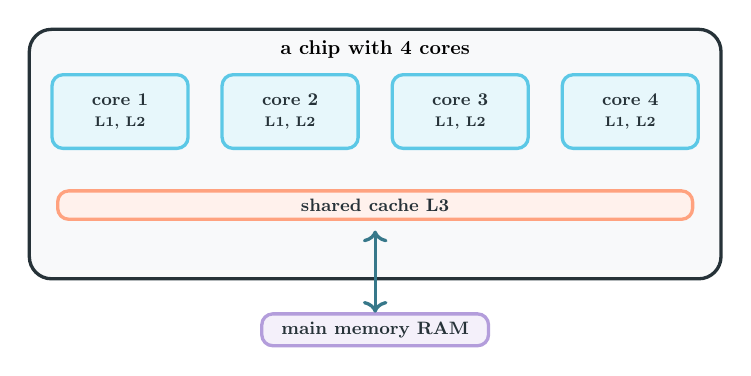
\begin{tikzpicture}[scale=0.72, transform shape, core/.style={unit, minimum width=2.4cm, minimum height=1.3cm}]
        \draw[brandDark, very thick, rounded corners=8pt, fill=brandLight] (-6.1,-2.4) rectangle (6.1,2);
        \node[font=\bfseries] at (0,1.65) {a chip with 4 cores};
        \foreach \x/\i in {-4.5/1, -1.5/2, 1.5/3, 4.5/4} \node[core] at (\x,0.55) {core \i\\{\scriptsize L1, L2}};
        \node[unit=brandOrange, minimum width=11.2cm] at (0,-1.1) {shared cache L3};
        \node[unit=brandPurple, minimum width=4cm] (ram) at (0,-3.3) {main memory RAM};
        \draw[sahmT, <->] (0,-1.55) -- (ram);
    \end{tikzpicture}
    \end{center}
    A \textbf{core} is a full processor. A \textbf{thread} is a series of instructions that runs on its own.
\end{frame}

\begin{frame}{Hyper-Threading}
    \begin{itemize}
        \item One core runs \textbf{two threads}: when one waits, the other works.
        \item Our processor: 4 cores, seen as 8 logical processors.
        \item If both threads need the same unit, we gain almost nothing.
    \end{itemize}
\end{frame}

\begin{frame}{A test: the same work on 1, 2, 4 and 8 threads}
    \cfiles[firstline=18, firstnumber=18, lastline=26]{ch5/threads.c}
    \screen{ch5/threads.out}
    Each thread adds the square roots of its share of 400 million numbers.
\end{frame}

\begin{frame}{Reading the results}
    \begin{columns}
        \column{0.5\textwidth}
        \begin{center}
        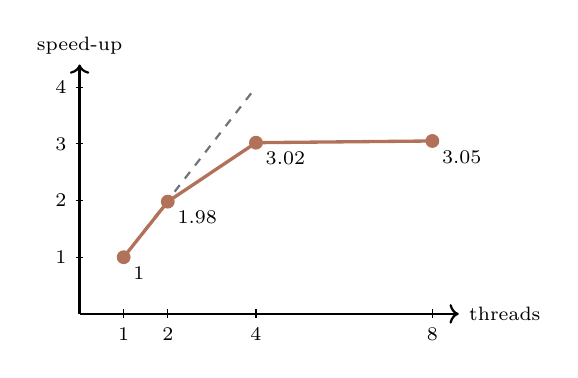
\begin{tikzpicture}[x=0.56cm, y=0.72cm]
            \draw[->, thick] (0,0) -- (8.6,0) node[right, font=\scriptsize] {threads};
            \draw[->, thick] (0,0) -- (0,4.4) node[above, font=\scriptsize] {speed-up};
            \foreach \y in {1,2,3,4} \draw (0.08,\y) -- (-0.08,\y) node[left, font=\scriptsize] {\y};
            \foreach \x in {1,2,4,8} \draw (\x,0.08) -- (\x,-0.08) node[below, font=\scriptsize] {\x};
            \draw[brandMuted, dashed, thick] (1,1) -- (4,4);
            \draw[orangeDeep, very thick] (1,1) -- (2,1.98) -- (4,3.02) -- (8,3.05);
            \foreach \x/\y in {1/1, 2/1.98, 4/3.02, 8/3.05} {
                \fill[orangeDeep] (\x,\y) circle (2.5pt);
                \node[font=\codefont\scriptsize, below right] at (\x,\y) {\y};
            }
        \end{tikzpicture}
        \end{center}
        \column{0.47\textwidth}
        \small
        \begin{itemize}
            \item 2 threads: 1.98, almost perfect.
            \item 4 threads: 3.02: heat and serial work.
            \item 8 threads: 3.05: only 4 real cores.
        \end{itemize}
    \end{columns}
\end{frame}

\begin{frame}{Amdahl's law}
    \begin{tbox}{\faLightbulb\quad If a part $p$ of the program is parallel, on $n$ cores:}
        \[ S(n) = \frac{1}{(1 - p) + \dfrac{p}{n}} \]
    \end{tbox}
    \begin{gbox}{\faShoePrints\quad $p = 0.9$}
        $S(4) = \frac{1}{0.1 + 0.225} \approx 3.08$ \quad (we measured 3.02!) \qquad $S(\infty) = \frac{1}{0.1} = 10$.
    \end{gbox}
\end{frame}

\begin{frame}{Benefits and challenges}
    \begin{center}
    \small
    \begin{tabularx}{0.95\linewidth}{|L|L|}
        \hline \ras{Benefits} & \ras{Challenges} \\ \hline
        more speed without a higher frequency & programs must use several threads \\ \hline
        less energy for the same work & the serial part limits the speed-up \\ \hline
        many programs run smoothly together & \textbf{synchronization} and \textbf{cache coherence} \\ \hline
    \end{tabularx}
    \end{center}
    \begin{obox}{\faExclamationTriangle\quad Synchronization}
        Two threads read x = 5 and both write 6: one increase is lost. We need locks or atomic instructions.
    \end{obox}
\end{frame}

\begin{frame}{Cache memory}
    \begin{tbox}{\faLightbulb\quad Definition}
        A small, fast memory near the processor that keeps a \textbf{copy} of recent data.
    \end{tbox}
    \begin{pbox}{\faSmile\quad Analogy}
        Desk (L1), bag (L2), cupboard (L3), library (RAM).
    \end{pbox}
\end{frame}

\begin{frame}{The memory hierarchy}
    \begin{center}
    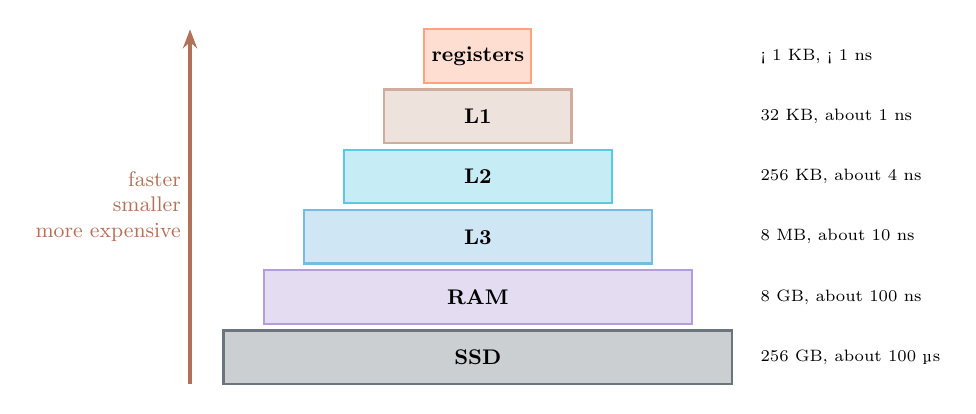
\begin{tikzpicture}[scale=0.85, transform shape]
        \foreach \y/\w/\t/\c/\d in {
            3.6/1.6/{registers}/brandOrange/{< 1 KB, < 1 ns},
            2.7/2.8/{L1}/brandOrange!70!brandTeal/{32 KB, about 1 ns},
            1.8/4.0/{L2}/brandTeal/{256 KB, about 4 ns},
            0.9/5.2/{L3}/brandTeal!70!brandPurple/{8 MB, about 10 ns},
            0.0/6.4/{RAM}/brandPurple/{8 GB, about 100 ns},
            -0.9/7.6/{SSD}/brandMuted/{256 GB, about 100 µs}} {
            \fill[\c!35, draw=\c, thick] (-\w/2,\y) rectangle (\w/2,\y+0.8);
            \node[font=\small\bfseries] at (0,\y+0.4) {\t};
            \node[font=\scriptsize, anchor=west] at (4.1,\y+0.4) {\d};
        }
        \draw[sahmO] (-4.3,-0.9) -- (-4.3,4.4) node[midway, left, font=\small, align=right] {faster\\smaller\\more expensive};
    \end{tikzpicture}
    \end{center}
\end{frame}

\begin{frame}{A test: we can see the memory levels}
    \begin{columns}
        \column{0.3\textwidth}
        \screen{ch5/latency.out}
        \column{0.67\textwidth}
        \begin{center}
        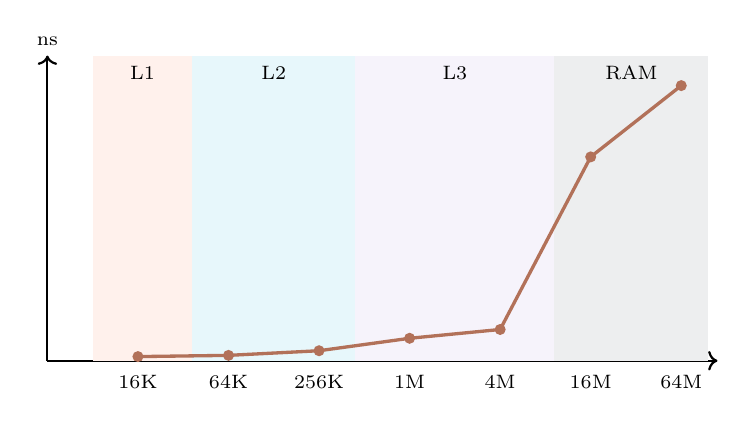
\begin{tikzpicture}[x=1.15cm, y=0.031cm]
            \draw[->, thick] (0,0) -- (7.4,0);
            \draw[->, thick] (0,0) -- (0,125) node[above, font=\scriptsize] {ns};
            \foreach \x/\t in {1/16K, 2/64K, 3/256K, 4/1M, 5/4M, 6/16M, 7/64M}
                \node[font=\codefont\scriptsize, below] at (\x,-2) {\t};
            \fill[brandOrange!15] (0.5,0) rectangle (1.6,125); \node[font=\scriptsize] at (1.05,118) {L1};
            \fill[brandTeal!15] (1.6,0) rectangle (3.4,125); \node[font=\scriptsize] at (2.5,118) {L2};
            \fill[brandPurple!12] (3.4,0) rectangle (5.6,125); \node[font=\scriptsize] at (4.5,118) {L3};
            \fill[brandMuted!12] (5.6,0) rectangle (7.3,125); \node[font=\scriptsize] at (6.45,118) {RAM};
            \draw[orangeDeep, very thick] (1,1.7) -- (2,2.2) -- (3,4.1) -- (4,9.2) -- (5,12.8) -- (6,83.5) -- (7,112.7);
            \foreach \x/\y in {1/1.7, 2/2.2, 3/4.1, 4/9.2, 5/12.8, 6/83.5, 7/112.7} \fill[orangeDeep] (\x,\y) circle (2pt);
        \end{tikzpicture}
        \end{center}
    \end{columns}
    From 1.7 ns (L1) to 113 ns (RAM): \textbf{65 times} slower.
\end{frame}

\begin{frame}{Locality: why caches work}
    \begin{itemize}
        \item \textbf{Temporal locality}: data used now will be used again soon.
        \item \textbf{Spatial locality}: after one address, we read the nearby ones.
    \end{itemize}
    \begin{tbox}{\faLightbulb\quad Cache line}
        The cache moves blocks of \textbf{64 bytes}: reading \code{t[0]} also brings \code{t[1]} to \code{t[15]}.
    \end{tbox}
\end{frame}

\begin{frame}{A test: row by row or column by column?}
    \begin{columns}[T]
        \column{0.66\textwidth}
        \cfiles[firstline=23, firstnumber=23, lastline=32]{ch5/locality.c}
        \screen{ch5/locality.out}
        \column{0.32\textwidth}
        \small
        \begin{itemize}
            \item C stores \textbf{row after row}.
            \item Columns: a new cache line every read.
            \item \textbf{33 times slower}!
        \end{itemize}
    \end{columns}
\end{frame}

\begin{frame}{Hits, misses, average time}
    \begin{tbox}{\faLightbulb\quad Average access time}
        \centering $h \times t_{cache} + (1 - h) \times t_{RAM}$ \qquad ($h$ = hit rate)
    \end{tbox}
    \begin{gbox}{\faShoePrints\quad $t_{cache} = 1$ ns, $t_{RAM} = 100$ ns}
        $h = 90\%$: 10.9 ns. \qquad $h = 99\%$: 1.99 ns, more than 5 times faster.
    \end{gbox}
\end{frame}

\begin{frame}{Mapping: where does a block go?}
    \begin{center}
    \small
    \begin{tabularx}{0.95\linewidth}{|>{\centering\arraybackslash}p{3cm}|L|L|}
        \hline \ras{Kind} & \ras{Rule} & \ras{Note} \\ \hline
        direct mapped & one possible line & simple, but conflicts \\ \hline
        fully associative & any line & few conflicts, costly search \\ \hline
        set associative & any of $k$ lines in a set & used in modern processors \\ \hline
    \end{tabularx}
    \end{center}
    Replacement: \textbf{LRU} (least recently used). Writing: \textbf{write-back} (fast) or write-through (simple).
\end{frame}

\begin{frame}{Splitting an address (direct mapped)}
    \small 1 KB cache, 16-byte lines, 16-bit addresses: 64 lines (6 bits), 16 bytes (4 bits), tag = 6 bits.
    \begin{center}
    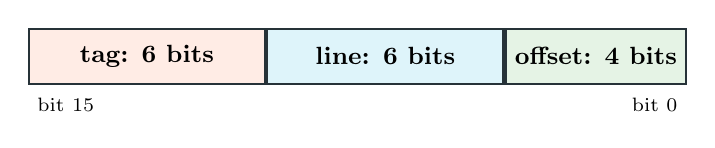
\begin{tikzpicture}[f/.style={draw=brandDark, thick, minimum height=0.7cm, font=\small\bfseries}]
        \node[f, minimum width=3cm, fill=brandOrange!20] (t) at (0,0) {tag: 6 bits};
        \node[f, minimum width=3cm, fill=brandTeal!20, anchor=west] (l) at (t.east) {line: 6 bits};
        \node[f, minimum width=2.2cm, fill=brandGreen!20, anchor=west] (o) at (l.east) {offset: 4 bits};
        \node[font=\codefont\scriptsize, below=1pt of t.south west, anchor=north west] {bit 15};
        \node[font=\codefont\scriptsize, below=1pt of o.south east, anchor=north east] {bit 0};
    \end{tikzpicture}
    \end{center}
    \begin{gbox}{\faShoePrints\quad $\hex{1A2C} = \bin{000110\,100010\,1100}$}
        tag = 6, line = 34, offset = 12.
    \end{gbox}
\end{frame}

\begin{frame}{Practice}
    \begin{obox}{\faEdit\quad Try it}
        \begin{enumerate}
            \item $p = 0.75$: maximum speed-up? \hfill \textcolor{brandMuted}{4}
            \item 2 ns cache, 80 ns RAM, 95\% hits: average? \hfill \textcolor{brandMuted}{5.9 ns}
            \item 4 KB cache, 32-byte lines, 32-bit addresses: tag bits? \hfill \textcolor{brandMuted}{20}
        \end{enumerate}
    \end{obox}
\end{frame}

\begin{frame}{Summary}
    \begin{tbox}{\faCheckCircle\quad Remember}
        \begin{itemize}
            \item More cores, not more GHz; Amdahl limits the gain.
            \item Memory: small and fast near, big and slow far.
            \item Read data in order: locality is speed.
        \end{itemize}
    \end{tbox}
\end{frame}

\end{document}
